\documentclass{article}
\usepackage{amsmath, amssymb, mdwlist, graphicx, hyperref}
\usepackage{listings,color}
\usepackage{wrapfig}
\usepackage[usenames,dvipsnames]{xcolor}
\definecolor{gray}{rgb}{0.97,0.97,0.97}
\lstset{%
language=Python,%
%backgroundcolor=\color{gray},
emph={putpixel},
emphstyle=\bf,
tabsize=4,
framesep=5pt,
mathescape=true,
xleftmargin=2cm,
xrightmargin=2cm,
frame=lines,
%basicstyle=\ttfamily,
%keywordstyle=\color{Blue},
%commentstyle=\color{OliveGreen},
%stringstyle=\color{MidnightBlue},
columns=flexible,
%showstringspaces=false
}

\newcommand{\mpar}[1]{\marginpar{\textit{#1}}}
\newcommand{\norm}[1]{\Vert #1 \Vert}
\DeclareMathOperator{\argmax}{argmax}
\DeclareMathOperator{\argmin}{argmin}
\newenvironment{solution}{\paragraph{Solution.}$\,$ }{\vskip 3mm\hrule}
\newenvironment{exercise}[2]{\begin{verse}\textbf{Exercise #1 (#2pt).} }{
\end{verse}\medskip}
\newcommand{\bbR}{\mathbb{R}}
\newcommand{\bw}{\mathbf{w}}
\newcommand{\bx}{\mathbf{x}}
\newcommand{\bd}{\mathbf{d}}
\newcommand{\bb}{\mathbf{b}}
\newcommand{\by}{\mathbf{y}}
\newcommand{\bzero}{\mathbf{0}}
\newcommand{\bz}{\mathbf{z}}
\newcommand{\bSigma}{\mathbf{\Sigma}}
\newcommand{\bp}{\mathbf{p}}
\newcommand{\bm}{\mathbf{m}}
\newcommand{\bc}{\mathbf{c}}
\newcommand{\bM}{\mathbf{M}}
\newcommand{\bK}{\mathbf{K}}
\newcommand{\bD}{\mathbf{D}}
\newcommand{\bA}{\mathbf{A}}
\newcommand{\bX}{\mathbf{X}}
\newcommand{\bY}{\mathbf{Y}}
\newcommand{\bR}{\mathbf{R}}
\newcommand{\bI}{\mathbf{I}}
\newcommand{\bS}{\mathbf{S}}
\newcommand{\bT}{\mathbf{T}}
\newcommand{\balpha}{\boldsymbol{\alpha}}
\newcommand{\pt}[2]{\left(\begin{array}{c}#1\\#2\end{array}\right)}

\begin{document}
\title{MTAT.03.015 Computer Graphics (Fall 2013)\\
Exercise session IV: Introduction to OpenGL}
\author{Konstantin Tretyakov, Ilya Kuzovkin}
\date{September 30, 2013}
\maketitle

OpenGL is a graphics API or, to put it slightly differently, an interface to the capabilities of the graphics hardware. OpenGL is not language-specific and can be used from most programming languages. We shall be programming in C, as before.

As usual, the base code is provided in the \texttt{practice04.zip} archive on the course website\footnote{Alternatively, all lecture slides and practice session materials are also available on Github: \url{http://github.org/konstantint/ComputerGraphics2013}}. Download, unpack and open it. You will need to submit your solution as a zipped archive file.

\section*{GLUT and OpenGL}
OpenGL is a purely graphics-oriented API. There are no functions in it that are related to such tasks as creating windows or receiving keyboard and mouse input. Such operations should be done by external means (e.g. using operating system calls).

For example, you can create a window using Allegro (like we did in the previous sessions) and then use OpenGL functions to draw on it. Instead of Allegro, however, we shall be using the FreeGLUT \emph{(Free GL Utility Toolkit)} library to create windows and process events, as it is somewhat more lightweight.

\begin{verse}
\textbf{Note:} The OpenGL library and headers are nearly always provided with the operating system and the development environment. The FreeGLUT library for Windows is bundled with the practice session materials. Users of Linux systems should install it, together with the GLU utility library by running
\begin{verbatim}
     apt-get install freeglut3-dev libglu-dev
\end{verbatim}
on Debian-based systems, or something similar for other distributions.

\noindent
On Mac you should install \texttt{freeglut} from MacPorts:
\begin{verbatim}
     sudo port install freeglut
\end{verbatim}
then add \texttt{/opt/local/include} to the compiler search path, \texttt{/opt/local/lib/} to the linker search path, and link with \texttt{glut} and \texttt{OpenGL.framework}. 
\end{verse}

Open the project \verb#1_HelloOpenGL# in CodeBlocks and study the code. Hopefully you will recognize the familiar structure of initializing the program, defining event handlers, and running the event loop, which will periodically invoke the event handlers and the display routine.

Play a bit with the code. Find the place where you can specify your own model-view matrix for the triangle scene and see how the use of \texttt{glTranslate}, \texttt{glRotate} and \texttt{glScale} functions influences the position of the triangle.

\begin{exercise}{1}{0.5} 
Make the triangle rotate slowly around the point $(0, 0.5)$.

Hint: \verb#glutGet(GLUT_ELAPSED_TIME)# returns the time elapsed since the program was started in milliseconds, as an \texttt{int}.
\end{exercise}

\begin{exercise}{2}{0.5} 
In the second scene a tiny ``tree'' with one branch and two leaves is being drawn. Your task is to modify the code so that the tree resembles the one below:
\begin{center}
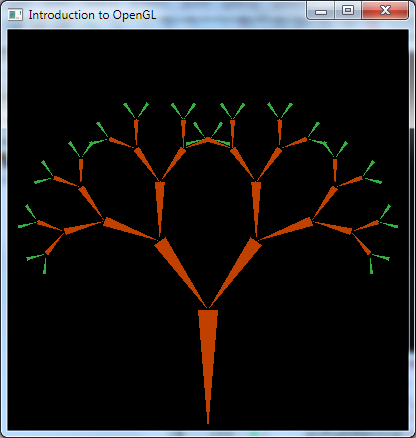
\includegraphics[width=0.75\textwidth]{tree.png}
\end{center}

Hint: Your new version of \verb#draw_tree# will become recursive and will take a parameter: \verb#draw_tree(int level)#.
\end{exercise}

\section*{3D Graphics}
Although the previous two exercises were two-dimensional, OpenGL is an inherently three-dimensional system. We were simply drawing everything in the plane $z=0$, which happens to be the projection plane. Try adding a rotation around the $x$ axis to any of the previous examples and see what happens.

Now, however, let us examine a purely three-dimensional example. Open the project file \verb#2_Cube#. Study the code. Note that it uses perspective projection and the z-buffer algorithm -- something that will be covered in the upcoming lectures. So far just take the provided set up for granted.

\begin{exercise}{3}{0.5}
Complete the implementation of \verb#draw_cube# so that the complete cube is drawn. Also, currently the cube is rotating on its own. Make it possible to rotate the cube interactively using the mouse (the exact behaviour of this interaction is up to you to choose, but even the simplest solution will do).
\end{exercise}


\begin{exercise}{4}{1}
Finally, open the project \verb#3_Solar#. Your task here is to implement a simple visualization of the Solar system. As a minimum, you should add four planets (Mercury, Venus, Earth and the Moon), making sure each planet rotates along its own circular orbit at its own pace.

You are encouraged (although not enforced) to make the model more realistic by ensuring the orbital periods for the planets are correct. You can also add more planets and set the view transformation to something better than what is given, if you wish.
\end{exercise}

Note that GLUT provides you with a bunch of pre-made primitive rendering functions, such as \texttt{glutSolidSphere}, that emit the constituent triangles as necessary. In fact, if you needed to draw a solid-color cube in Exercise 3, you could get away by simply using \texttt{glutSolidCube}.

\begin{exercise}{5*}{1-2}
Implement a three dimensional version of the ``jumping guy game'' from the first practice session. The character must be able to walk on a square field. The player should be able to control the character using the arrow keys (move around) and the spacebar (jump).

Hint: You do not have to make the character very detailed. Something like a \texttt{glutSolidCylinder} combined with a \texttt{glutSolidSphere} will do. If you want, though, you can try finding (or making) a suitable 3D model in the Wavefront .obj format and using it as shown in \verb#4_Object#.

Hint: To respond to arrow keys you will need \texttt{glutSpecialFunc}, rather than \texttt{glutKeyboardFunc}.

Something simple (e.g. making the guy in \verb#4_Object# move around) gives 1 point. Displays of creativity are awarded with an additional point.
\end{exercise}

\begin{exercise}{6*}{0.5}
Make the tree from the exercise 2 three-dimensional. Use appropriately-sized \texttt{glutSolidCylinder}s as the branches, simple triangles for the leaves, and make the branching topology three-dimensional (i.e. rather than having two branches go ``left'' and ``right'', have three or more branches at each level go in various directions).

Do not forget that you need to enable perspective projection and depth buffer.
\end{exercise}

\end{document}
